\uuid{tjkm}
\exo7id{6974}
\titre{exo7 6974}
\auteur{blanc-centi}
\organisation{exo7}
\datecreate{2014-05-06}
\video{pT2xX0g3eDA}
\isIndication{false}
\isCorrection{true}
\chapitre{Fonctions circulaires et hyperboliques inverses}
\sousChapitre{Fonctions circulaires inverses}
\module{Analyse}
\niveau{L1}
\difficulte{}

\contenu{
\texte{
Soit $z=x+iy$ un nombre complexe, où $x=\Re z$ et $y=\Im z$. 
On sait que si $z$ est non nul, on peut l'écrire de façon unique sous la forme 
$z=x+iy=re^{i\theta}$, où $\theta\in]-\pi,\pi]$ et $r=\sqrt{x^2+y^2}$. 
\begin{center}
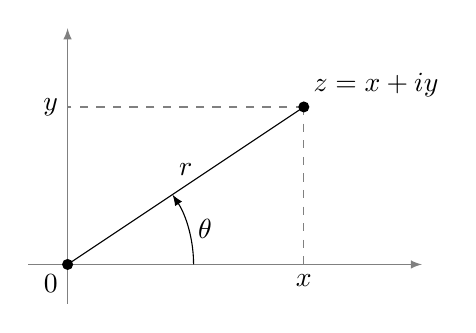
\begin{tikzpicture}[scale=1]
      \draw[->,>=latex, gray] (-0.5,0)--(4.5,0);
       \draw[->,>=latex, gray] (0,-0.5)--(0,3);

      \coordinate (A) at (3,2);
      \coordinate (Ax) at (3,0);
      \coordinate (Ay) at (0,2);

       \draw[thin] (0,0)--(A) node[midway,above] {$r$};
       \draw[dashed,gray] (A)--(Ax);
       \draw[dashed,gray] (A)--(Ay);

       \fill (A) circle (2pt);
       \fill (0,0) circle (2pt);

       \node at (0,0) [below left] {$0$}; 
       \node at (A) [above right] {$z=x+iy$}; 
       \node at (Ax) [below] {$x$}; 
       \node at (Ay) [left] {$y$};
       
       \draw[->,>=latex] (0:1.6) arc (0:33.69:1.6);
       \node[right] at (16.5:1.6) {$\theta$};
\end{tikzpicture}  
\end{center}
}
\begin{enumerate}
    \item \question{Montrer que si $x>0$, alors $\theta=\Arctan\frac{y}{x}$.}
\reponse{Si $x>0$, alors $\frac{y}{x}$ est bien défini et $\Arctan\frac{y}{x}$ aussi. 
Comme $x=r\cos\theta$ et $y=r\sin\theta$, on a bien $\frac{y}{x}=\tan\theta$.
Puisque par hypothèse $\theta\in]-\pi,\pi]$ et que l'on a supposé $x>0$,
alors $\cos\theta>0$.
Cela implique $\theta\in]-\frac{\pi}{2},\frac{\pi}{2}[$. 
Donc $\theta=\Arctan(\tan\theta)=\Arctan\frac{y}{x}$. (Attention ! Il est important
d'avoir $\theta\in]-\frac{\pi}{2},\frac{\pi}{2}[$ pour considérer l'identité 
$\Arctan(\tan\theta) = \theta$.)}
    \item \question{Montrer que si $\theta\in]-\pi,\pi[$, alors 
$\theta=2\Arctan\left(\frac{\sin\theta}{1+\cos\theta}\right)$.}
\reponse{Si $\theta\in]-\pi,\pi[$ alors $\frac{\theta}{2}\in]-\frac{\pi}{2},\frac{\pi}{2}[$, 
donc $\frac{\theta}{2}=\Arctan\left(\tan\frac{\theta}{2}\right)$. Or 
$$\frac{\sin\theta}{1+\cos\theta}=
\frac{2\cos\frac{\theta}{2}\sin\frac{\theta}{2}}{1+\big(2\cos^2\left(\frac{\theta}{2}\right)-1\big)}
=\frac{\sin\frac{\theta}{2}}{\cos\frac{\theta}{2}}=\tan\frac{\theta}{2}$$
d'où $\frac\theta2=\Arctan\left(\tan\frac{\theta}{2}\right)=\Arctan\left(\frac{\sin\theta}{1+\cos\theta}\right)$.}
    \item \question{En déduire que si $z$ n'est pas réel négatif ou nul, on a l'égalité
$$\theta=2\Arctan\left(\frac{y}{x+\sqrt{x^2+y^2}}\right).$$}
\reponse{Remarquons que $z=x+iy$, supposé non nul, est un nombre réel négatif si et seulement si 
($x=r\cos\theta< 0$ et $y=r\sin\theta=0$), c'est-à-dire $\theta=\pi$. 
Par conséquent, dire que $z$ n'est pas réel négatif ou nul signifie que 
$\theta\in]-\pi,\pi[$. On a alors $x+\sqrt{x^2+y^2}\not=0$ (sinon, on aurait $\sqrt{x^2+y^2}=-x$ 
et donc $y=0$ et $x\le 0$) et 
$$\frac{y}{x+\sqrt{x^2+y^2}}=\frac{r\sin\theta}{r\cos\theta+r}=\frac{\sin\theta}{1+\cos\theta}.$$
Par la question précédente :
$$\theta = 2\Arctan\left(\frac{\sin\theta}{1+\cos\theta}\right) = 2\Arctan\left(\frac{y}{x+\sqrt{x^2+y^2}}\right).$$}
\end{enumerate}
}
